\documentclass[11pt,a4paper]{article}
\usepackage{fontspec}
\setmainfont{TeX Gyre Pagella}
\newfontfamily\headfont{Inter}[UprightFont=*-ExtraBold,BoldFont=*-ExtraBold,Extension=.otf,Path=/usr/share/fonts/opentype/inter/]
\usepackage[a4paper,margin=2.3cm]{geometry}
\usepackage{graphicx,booktabs,float,caption,array,xcolor,longtable}
\usepackage{xurl}
\usepackage[hidelinks]{hyperref}
\usepackage{titlesec}
\usepackage[round]{natbib}
\usepackage{setspace}
\setstretch{1.05}
\renewcommand{\topfraction}{0.9}
\renewcommand{\bottomfraction}{0.8}
\renewcommand{\textfraction}{0.1}
\renewcommand{\floatpagefraction}{0.75}
\setlength{\parindent}{0pt}
\setlength{\parskip}{0.55em}
\titleformat{\section}{\headfont\Large}{\thesection}{0.8em}{}
\titleformat{\subsection}{\headfont\large}{\thesubsection}{0.8em}{}
\captionsetup{font=small,labelfont=bf}
\urlstyle{same}
\hypersetup{pdftitle={Every Battle in History},pdfauthor={Tristan Hotham}}


\begin{document}
\begin{center}
{\Large\bfseries Every Battle in History\par}
\vspace{0.4em}
{\large Five thousand years of battles in Wikidata: where war happened,\\the most fought-over places, and how skewed the record is\par}
\vspace{1.2em}
{\large Tristan Hotham\par}
\vspace{0.3em}
{\small Independent researcher\\
ORCID: 0000-0003-4931-9349\\
DOI: https://doi.org/10.5281/zenodo.23857870\par}
\vspace{0.8em}
2026
\end{center}

\begin{quote}
\small
\begin{center}\textbf{Abstract}\end{center}
Maps of ``every battle in history'' circulate widely, but rarely with dates, method or caveats. I map every Wikidata item that is an instance of battle or one of its subclasses: 20,202 items, of which 13,712 have both coordinates and a date, from a legendary battle placed in 3001 BCE to 2026. The record is overwhelmingly recent: 77\% of dated battles are after 1500 and 52\% after 1800, with the 19th century (3,714 battles) and the 20th (3,630) the best recorded. The spherical median of each century's battles, a ``centre of war'', lies in Greece in the 5th century BCE and in Italy under Rome, and from the 5th to the 19th century lies within 800 km of the Alps in every century but the 7th; it has moved to Syria in the 21st century. On an equal-area hexagonal grid the most fought-over region is Flanders, Artois and Brabant (369 battles in 17 centuries), while the longest fought-over hexagon is Jerusalem, Gaza and the coastal plain, with battles in 16 centuries. The best-recorded wars are the Second World War (864 battle items), the First (532) and the American Civil War (524). The record is strongly skewed: Europe has 51\% of mapped battles on 7\% of the world's land, coverage of some wars is extraordinarily dense, 7.1\% of items lack an English label, and only 79\% are labelled as battles at all. I argue that the map is best read as a map of the historical record as much as of war itself.

\textbf{Keywords:} battles; military history; Wikidata; Wikipedia; knowledge gaps; historical GIS; spatial analysis; open data
\end{quote}

\section{Introduction}
Maps that plot ``every battle in history'' are a familiar genre of online data visualisation. They are usually built from Wikidata or DBpedia, and they look alike: Europe dense with points, the eastern United States marked by the Civil War, and much of Africa, Asia and South America sparse. They are striking, but they are rarely dated, rarely explain what was counted, and almost never discuss how the underlying record was made.

This paper rebuilds that map carefully and asks four descriptive questions. How are recorded battles distributed through time? Where was the ``centre'' of recorded war in each century? Which places have been fought over most often, and for longest? And how skewed is the record by region, period, language and the way battles are classified? The data are Wikidata's battle items \citep{wikidata}, retrieved through the QLever endpoint \citep{qlever}, with an additional layer from English Wikipedia's list of battles by casualties \citep{wp_cas}. An interactive version, with a time slider, filters by war and kind of event, and the layers used here, is at \url{https://maps.tristanhotham.com/every-battle/}.

Wikidata is a collaboratively edited knowledge base closely tied to Wikipedia. Its coverage reflects the interests of its editors and of the Wikipedia language editions it draws on, and earlier work has documented strong geographical and gender gaps in Wikipedia and Wikidata \citep{graham,redi}. Battles are a useful test case because they are a well defined kind of event, recorded across thousands of years and in every region of the world, and because their geography is often read as if it were the geography of war.

\section{Data}
\textbf{Battle items.} I selected every Wikidata item that is an instance of battle (Q178561) or of any subclass of it, with its English label, the number of Wikipedia sitelinks (language editions with an article), its own coordinates (P625), its location (P276) with that location's label and coordinates, its point in time (P585) and start time (P580), and the label of any item it is ``part of'' (P361). The query returned 23,069 rows, one per combination of location and ``part of'' value, which reduce to 20,202 distinct items. Wikidata is released under CC0.

\textbf{Coordinates.} 9,626 items have their own coordinates. For another 5,142 I used the coordinates of the item's location; when an item has several locations I took the one closest to their median. Location coordinates can be those of a town, a region or a sea, so these points are less precise. In all, 14,768 items (73\%) have a point.

\textbf{Dates.} The year is the earliest point in time, else the earliest start time; 15,874 items (79\%) have one. The RDF export used by QLever writes years in astronomical numbering (year 0 is 1 BCE, $-216$ is 217 BCE), which I convert for display. Date precision was not exported, so a year may stand for a decade, a century or a millennium. Centuries are ordinal (the 19th century is 1801 to 1900), which places values such as 1300, Wikidata's encoding of the 13th century, in the right century. 13,712 items (68\%) have both a point and a date, and these form the main analysis set.

\textbf{Casualties.} English Wikipedia's ``List of battles by casualties'' (revision 1382711824, CC BY-SA 4.0) contains 709 rows in five tables: sieges and urban combat, major operations, classical formation battles, raids and sacks, and naval battles. I took the highest casualty figure in each row and matched rows to Wikidata items by English label and year.

\textbf{Geography.} Country and continent come from Natural Earth's 1:50m countries \citep{naturalearth}; city names for labels and search from Natural Earth populated places.

\section{Methods}
\textbf{Places and continents.} A battle takes the country whose outline contains its point, or for points at sea (1,369 of the mapped battles) the nearest country within 400 km. 43 battles further out are left without a continent. Russia west of the Urals and Turkey west of the Bosporus are counted as Europe.

\textbf{Kinds of event.} Wikidata's subclasses of battle include sieges, naval battles, skirmishes, assaults and many more, and the classes are used inconsistently. I classify items instead by the first matching word in their English label: battle; siege; skirmish or action; raid, attack or capture; bombing or bombardment; massacre; operation or offensive; and other or no English label (Table~\ref{tab:kinds}).

\textbf{Wars.} Each battle's war is the ``part of'' value with the most battles overall. Because Wikidata often records a theatre or campaign rather than a war, I grouped the theatres and campaigns of the two world wars into the wars themselves, only within 1914 to 1918 and 1939 to 1945.

\textbf{Centre of war.} For each century with at least 20 mapped battles I computed the spherical geometric median: the point on the sphere that minimises the sum of great-circle distances to the century's battles, found with Weiszfeld's algorithm in three dimensions. The median is more robust than the mean position, which on a sphere is pulled poleward when points are widely spread; but when battles fall in two distant clusters the median lands between them, in a place where no battle was fought.

\textbf{Hexagons and regions.} I counted battles on a grid of pointy-top hexagons in the Equal Earth projection (EPSG:8857; \citealp{equalearth}), so that each hexagon covers the same area: 9,353 km², about the size of Cyprus. To reduce the effect of where hexagon boundaries fall, I also built regions of seven hexagons (a hexagon and its six neighbours, 65,472 km²), chosen greedily by battle count with no overlap. Places were named from the battles and locations inside them. I ranked hexagons both by the number of battles and by the number of distinct centuries in which a battle took place.

\textbf{Bias.} I compare continents' shares of battles with their shares of the world's land (Natural Earth, excluding Antarctica, with the same Europe definition), and use sitelinks as a measure of how widely a battle is known.

\section{Results}
\subsection{Battles through time}
Figure~\ref{fig:centuries} shows battles per century. Only 3 are dated before 2000 BCE and 672 before 1 CE. The oldest is the Battle of Banquan of Chinese tradition, placed in 3001 BCE. Numbers rise slowly through the first millennium CE and steeply after 1500: 77\% of dated battles are after 1500 and 52\% after 1800. The 19th century has 3,714 battles, the 20th 3,630 and the 18th 1,823; the 19th and 20th together hold 46\%. Per year, the rate is 37.1 in the 19th century, 36.3 in the 20th and 35.4 in the 21st so far. The busiest year is 1944 (319 battles), followed by 1863 (256), and the busiest decade the 1940s (1,216).

\begin{figure}[tbp]\centering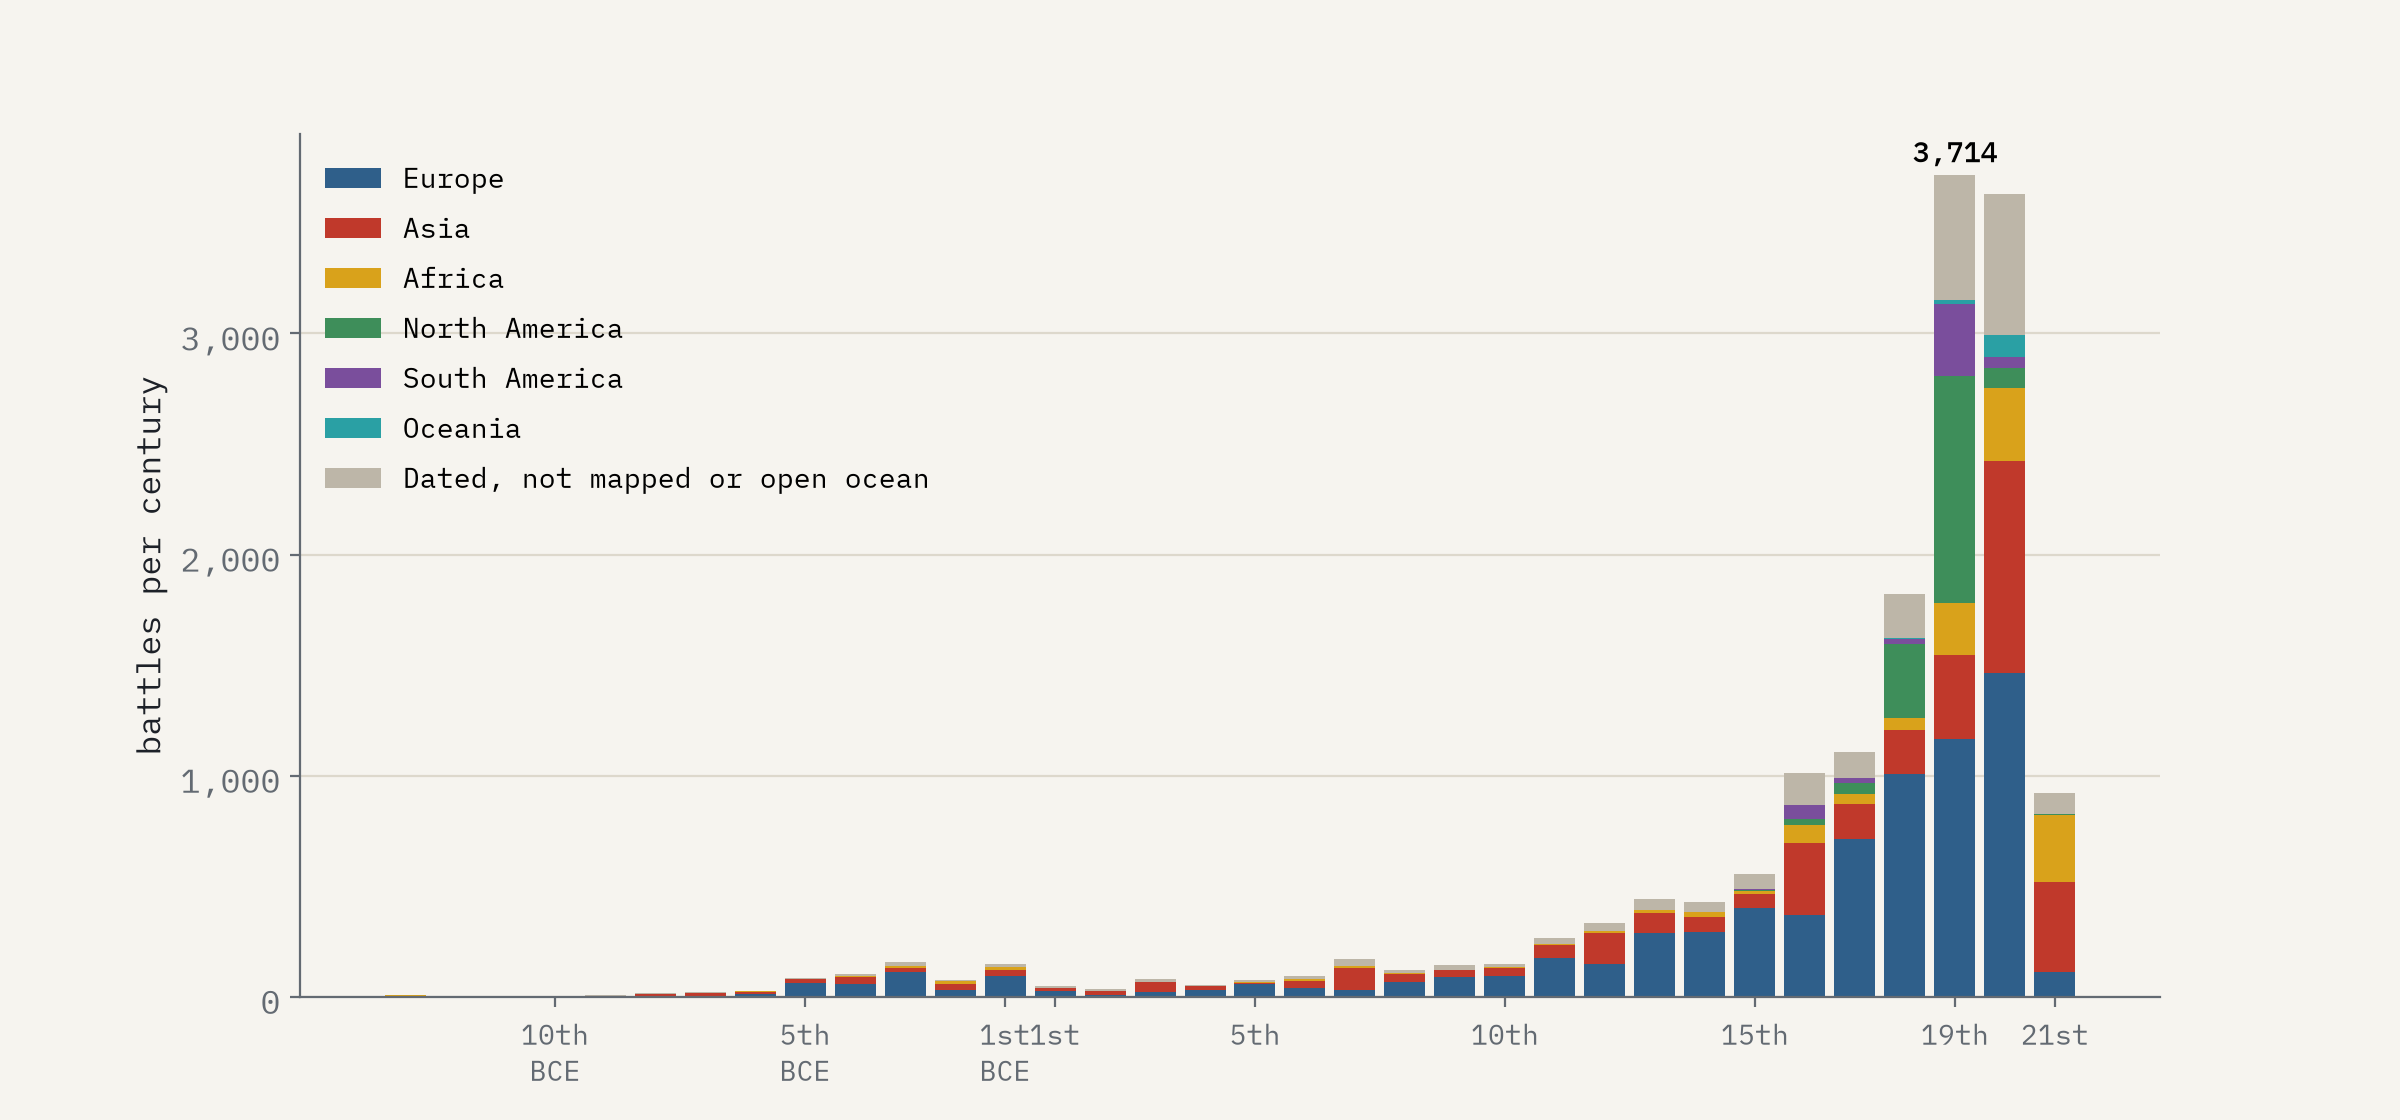
\includegraphics[width=\textwidth]{f_centuries.png}
\caption{Dated battles per century, 13th century BCE to 21st century (2001 to 2026), coloured by the continent of mapped battles.}\label{fig:centuries}\end{figure}

Figure~\ref{fig:world} maps every dated battle coloured by era, and Figure~\ref{fig:eras} shows each era separately on an equal-area hexagonal grid. Table~\ref{tab:eras} gives the continental shares by era.

\begin{figure}[tbp]\centering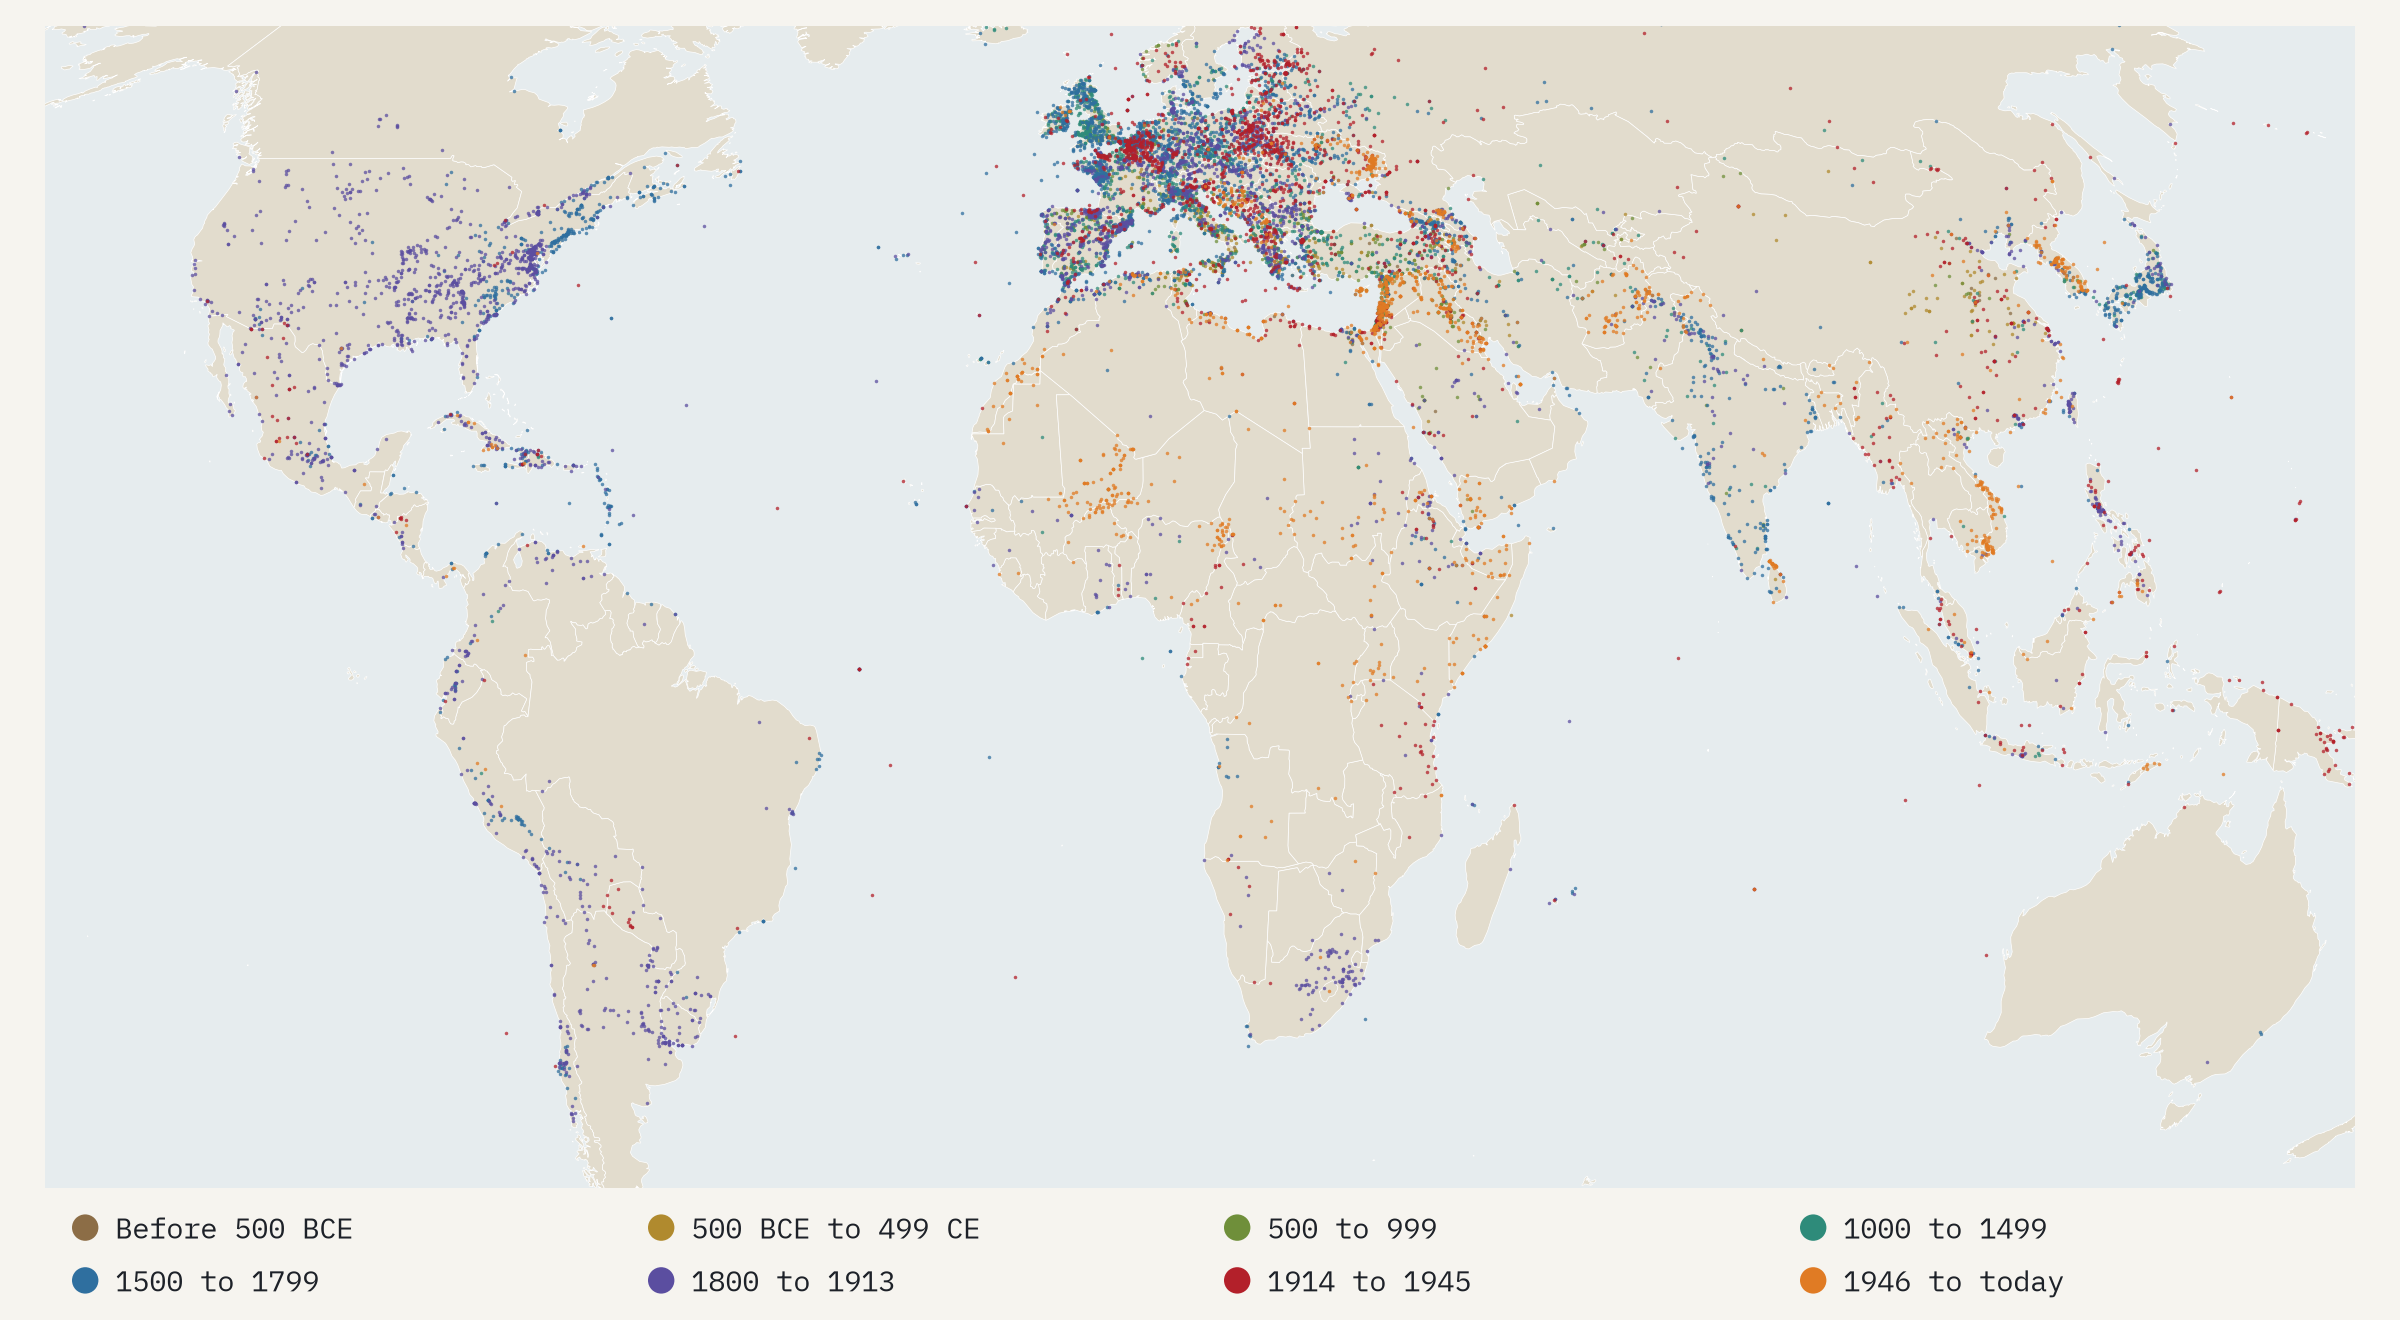
\includegraphics[width=\textwidth]{f_world.png}
\caption{Every mapped and dated battle item in Wikidata, coloured by era (Equal Earth projection).}\label{fig:world}\end{figure}

\begin{figure}[tbp]\centering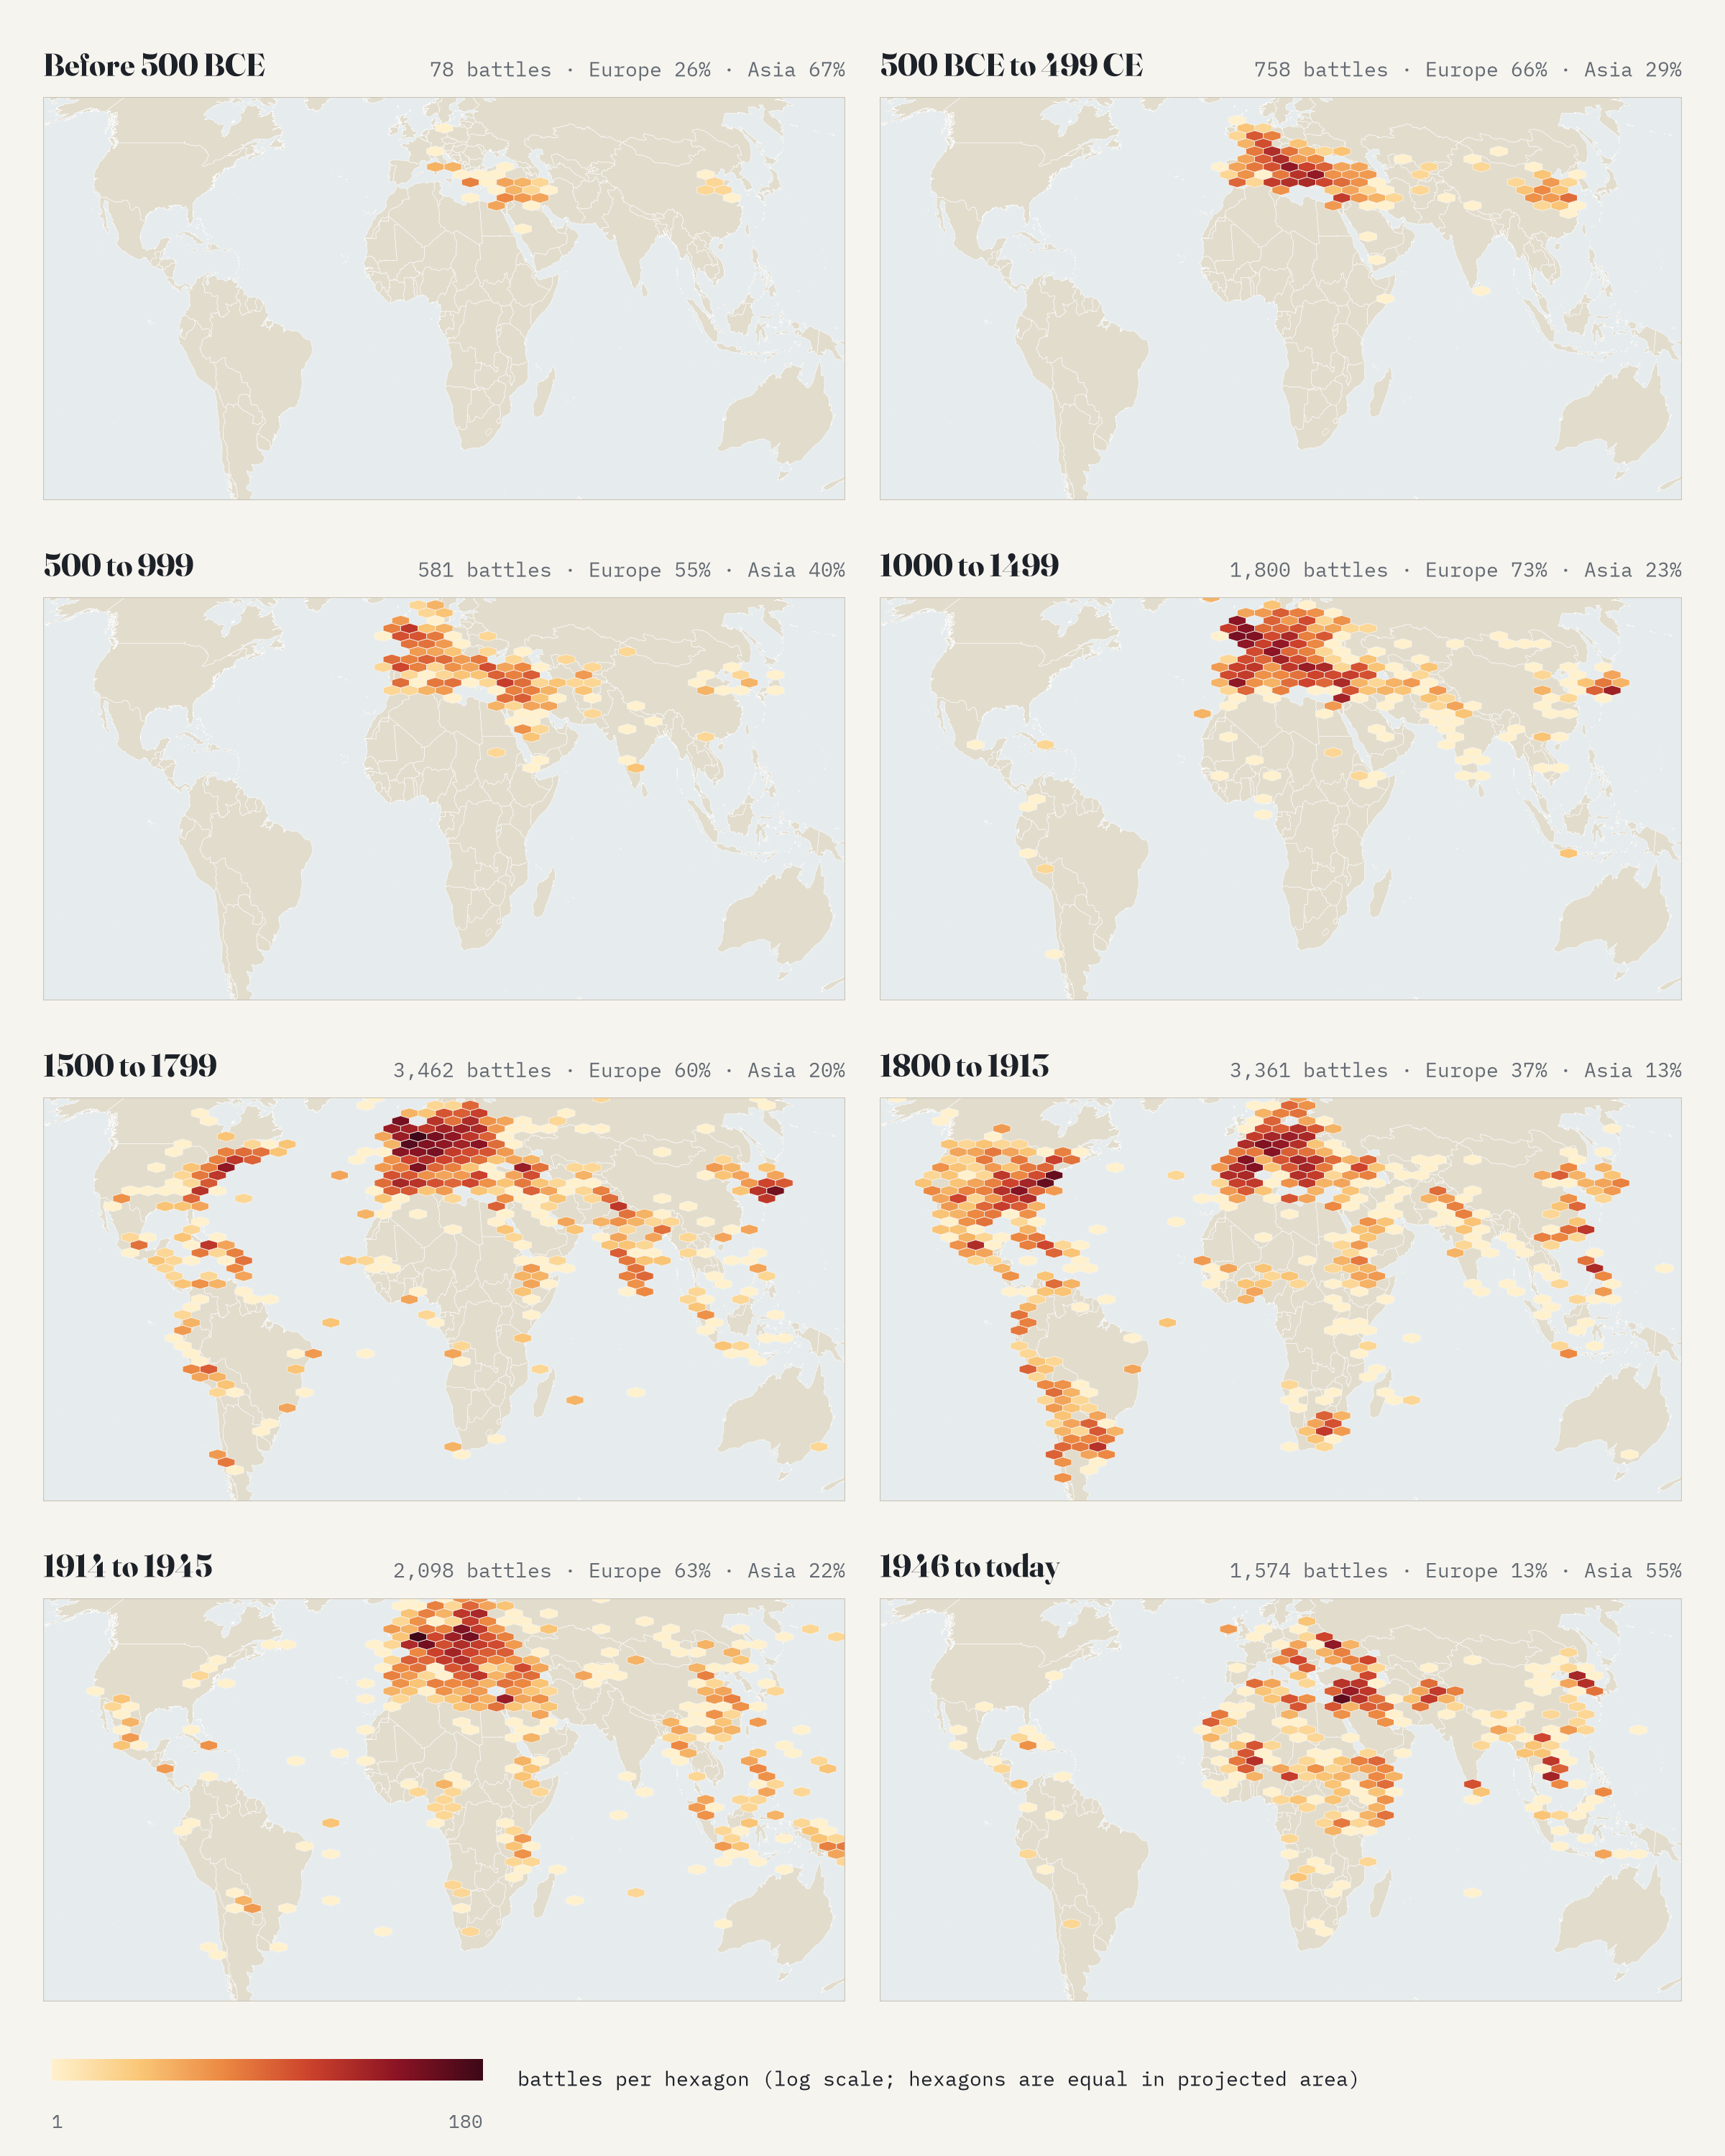
\includegraphics[width=\textwidth]{f_eras.png}
\caption{Battles by era, counted in hexagons (one log colour scale for all panels).}\label{fig:eras}\end{figure}

\begin{table}[tbp]\centering\small\caption{Battles by era: dated battles, mapped battles and the share of mapped battles by continent.}\label{tab:eras}\begin{tabular}{lrrrrrrrr}\toprule Era & Dated & Mapped & Europe & Asia & Africa & N. Am. & S. Am. & Oceania\\\midrule
Before 500 BCE & 99 & 78 & 26\% & 67\% & 8\% & 0\% & 0\% & 0\%\\
500 BCE to 499 CE & 862 & 758 & 66\% & 29\% & 5\% & 0\% & 0\% & 0\%\\
500 to 999 & 675 & 581 & 55\% & 40\% & 6\% & 0\% & 0\% & 0\%\\
1000 to 1499 & 2,021 & 1,800 & 73\% & 23\% & 4\% & 0\% & 0\% & 0\%\\
1500 to 1799 & 3,914 & 3,462 & 60\% & 20\% & 5\% & 12\% & 3\% & 0\%\\
1800 to 1913 & 3,950 & 3,361 & 37\% & 13\% & 8\% & 31\% & 10\% & 1\%\\
1914 to 1945 & 2,540 & 2,098 & 63\% & 22\% & 7\% & 2\% & 1\% & 5\%\\
1946 to today & 1,813 & 1,574 & 13\% & 55\% & 29\% & 1\% & 2\% & 0\%\\
\bottomrule\end{tabular}\end{table}

\subsection{The centre of war}
The centre of recorded war (Figure~\ref{fig:centre}, Table~\ref{tab:centres}) lies in Greece from the 6th to the 4th century BCE and in Italy for most of the Roman Republic. From the 5th to the 19th century CE it lies within 800 km of the middle of the Alps in every century except the 7th, moving between northern Italy, Austria, Switzerland, southern Germany, the Czech lands and northern France. The departures are informative. In the 2nd and 3rd centuries CE the median lies near the Caucasus and the Caspian because the record contains more Chinese battles than Roman ones (67\% of the 3rd century's mapped battles are in Asia), and half of that century's battles are more than 3,090 km from the median. In the 7th century the Arab conquests move it to Syria. In the 20th it lies in Romania, between the Western Front, the Eastern Front and the Middle East. In the 21st century it is in Syria, 1,883 km from its 20th-century position, with 49\% of mapped battles in Asia and 37\% in Africa.

\begin{figure}[tbp]\centering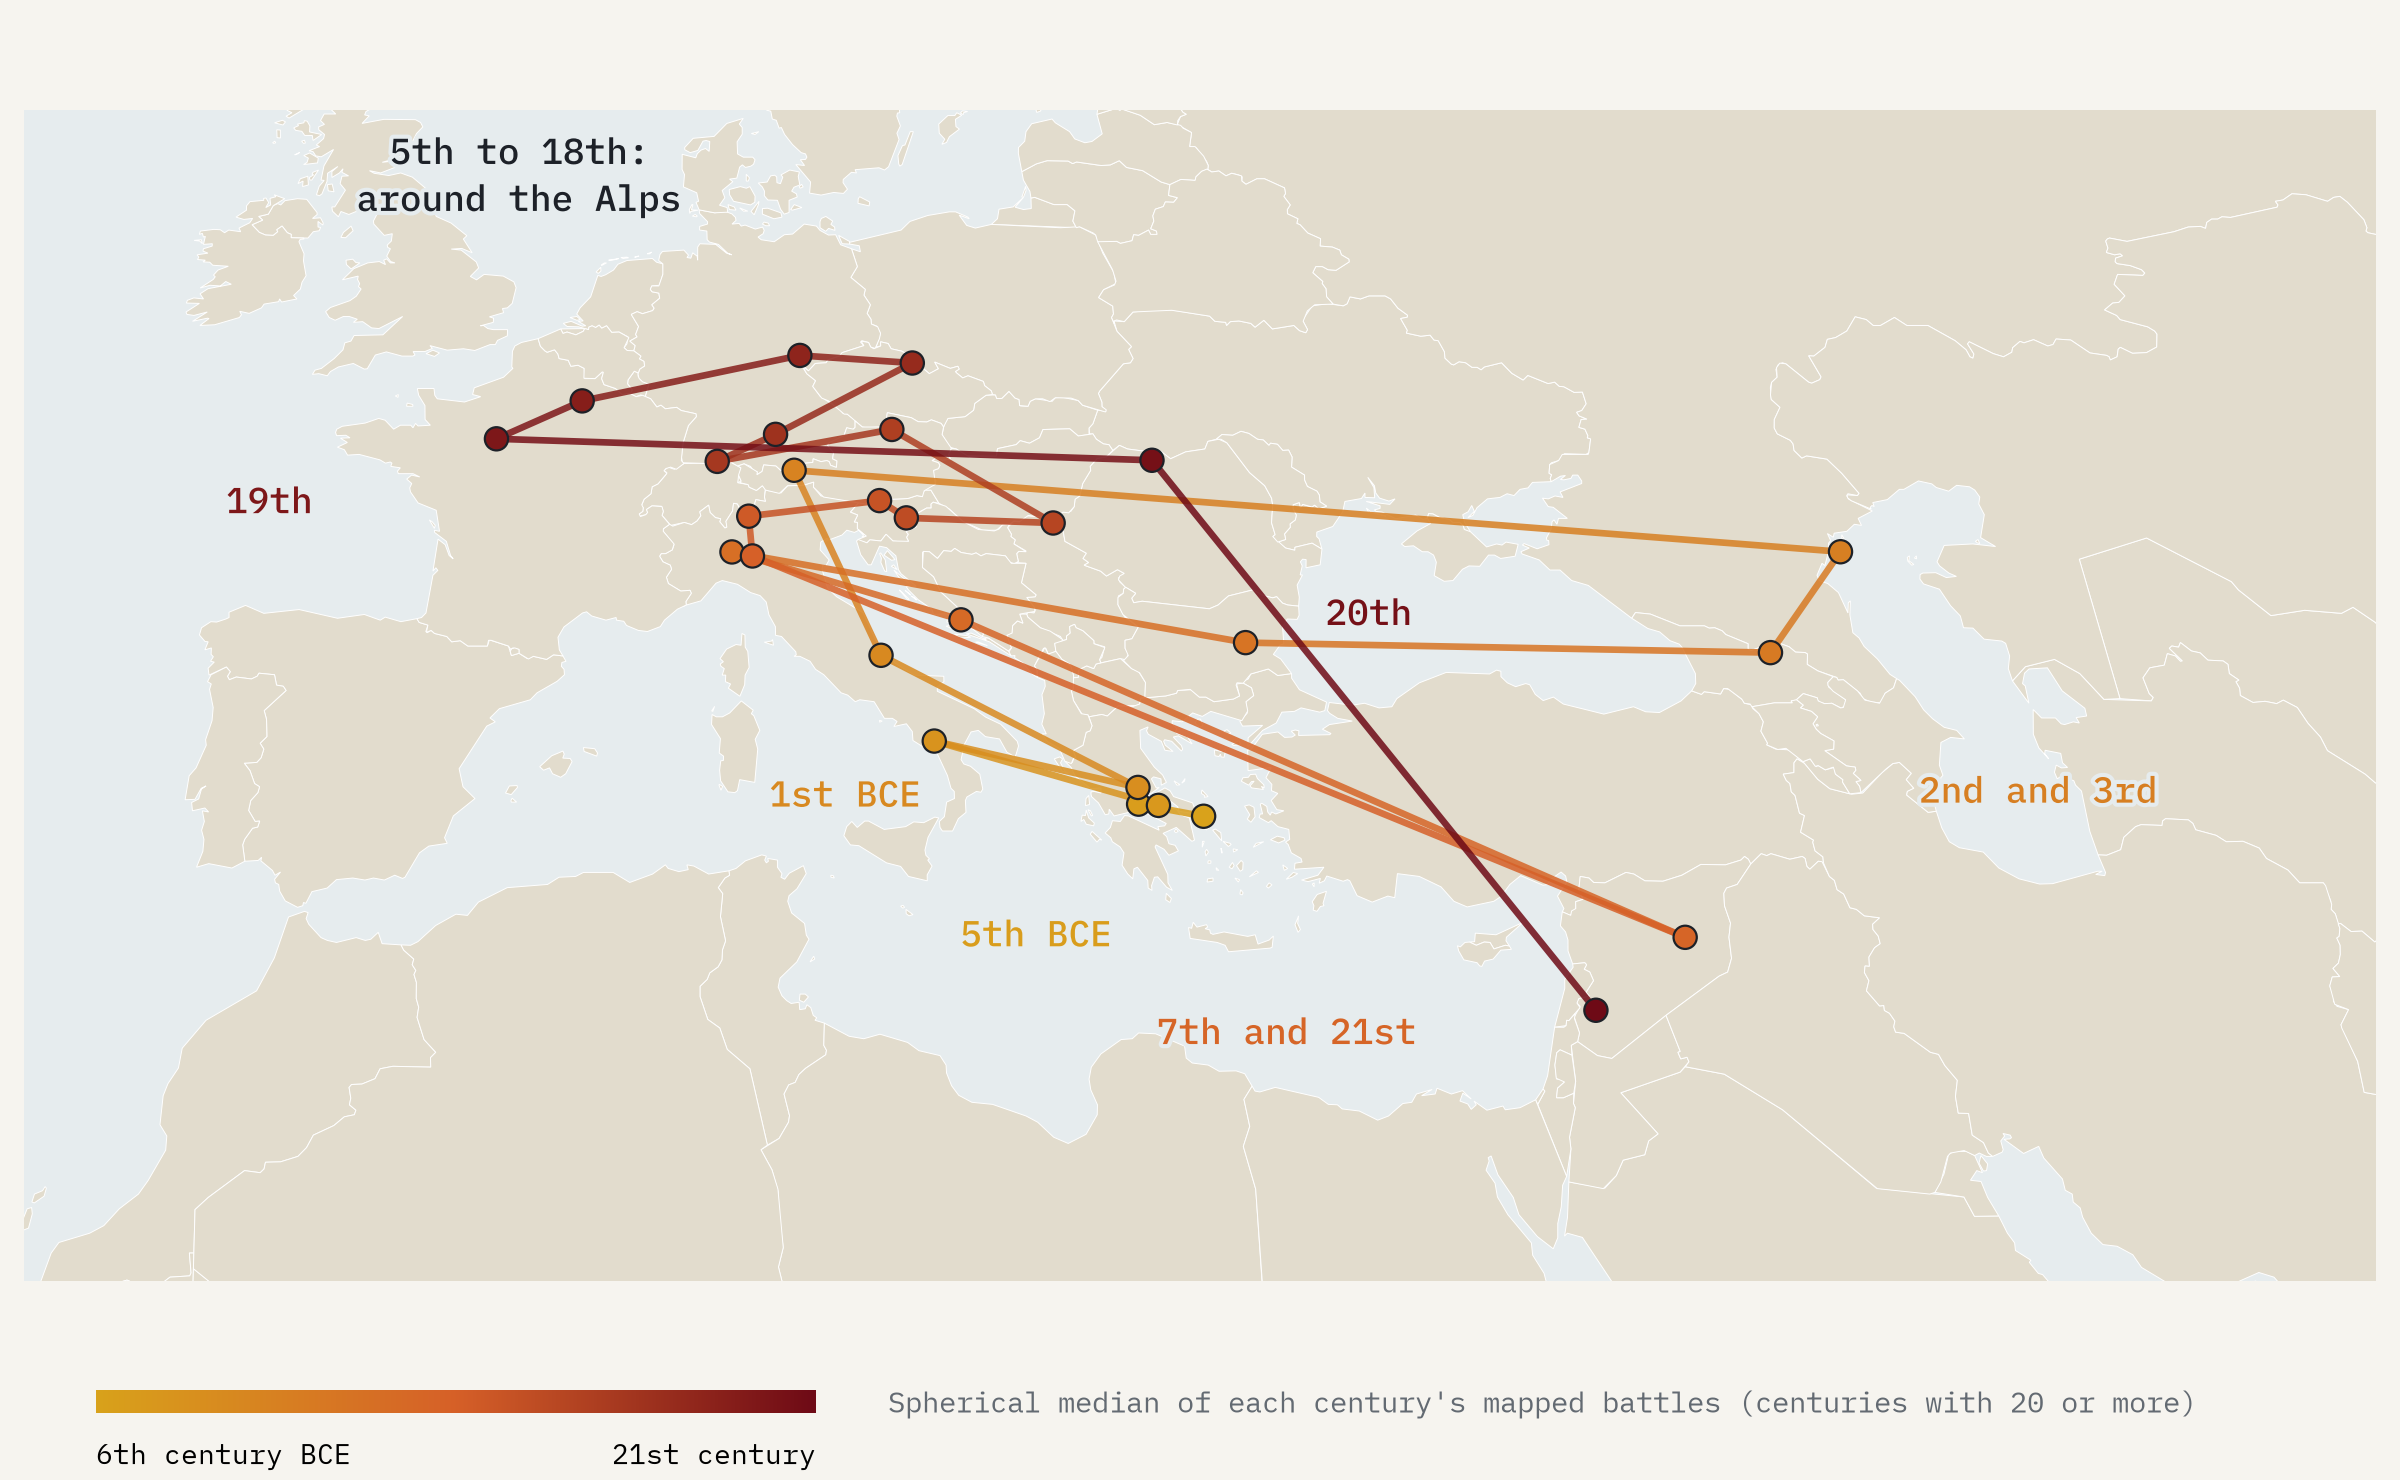
\includegraphics[width=\textwidth]{f_centre.png}
\caption{The centre of war: the spherical geometric median of each century's mapped battles, for centuries with 20 or more.}\label{fig:centre}\end{figure}

\begin{table}[tbp]\centering\small\caption{The centre of war: spherical geometric median of each century's mapped battles, and the distance within which half of them lie.}\label{tab:centres}\begin{tabular}{lrlr}\toprule Century & Battles & Centre in or near & Half within (km)\\\midrule
6th century BCE & 24 & Greece (sea) & 1,082\\
5th century BCE & 79 & Greece & 435\\
4th century BCE & 93 & Greece & 720\\
3rd century BCE & 140 & Italy & 587\\
2nd century BCE & 70 & Greece & 1,237\\
1st century BCE & 133 & Italy & 1,025\\
1st century & 41 & Austria & 897\\
2nd century & 25 & Russia (sea) & 3,307\\
3rd century & 67 & Georgia & 3,090\\
4th century & 47 & Bulgaria & 1,278\\
5th century & 66 & Italy & 703\\
6th century & 81 & Croatia (sea) & 1,607\\
7th century & 140 & Syria & 1,025\\
8th century & 107 & Italy & 1,400\\
9th century & 120 & Italy & 1,138\\
10th century & 133 & Austria & 1,420\\
11th century & 241 & Slovenia & 1,454\\
12th century & 299 & Romania & 1,888\\
13th century & 391 & Austria & 1,353\\
14th century & 383 & Switzerland & 1,257\\
15th century & 488 & Germany & 1,035\\
16th century & 867 & Czech Republic & 2,592\\
17th century & 994 & Germany & 1,219\\
18th century & 1,629 & France & 1,409\\
19th century & 3,156 & France & 6,190\\
20th century & 3,016 & Romania & 1,875\\
21st century & 828 & Syria & 2,069\\
\bottomrule\end{tabular}\end{table}

\subsection{The most fought-over places}
Flanders, Artois and Brabant is the most fought-over region: 369 battles across 17 centuries, from Caesar's campaign against the Belgae through the Battle of the Golden Spurs, the Eighty Years' War, Ramillies and Malplaquet, Waterloo and the battles of Ypres (Figure~\ref{fig:places}, Table~\ref{tab:regions}). Its busiest hexagon, Arras, Artois and southern Flanders, has 113 battles, the most of any. Among countries of 20,000 km² or more, Belgium has the most battles per unit area, 63.4 per 10,000 km² (195 battles). The top ten hexagons hold 5.0\% of mapped battles and the top hundred 24\%.

Ranked by duration rather than number, the leaders are in the Levant and Italy. Jerusalem, Gaza and the coastal plain has battles in 16 centuries, from 1025 BCE to 2025, and in all eight eras; only 2 hexagons do, the other being Baghdad. Milan, Pavia and the Adda has 16 centuries and Rome 15.

The second region, Western France, from the Vendée to Normandy (260 battles), is an artefact of uneven description as much as of war: 68\% of its battles belong to the War in the Vendée or the Chouannerie, which together have 191 battle items, more than the Thirty Years' War.

\begin{figure}[tbp]\centering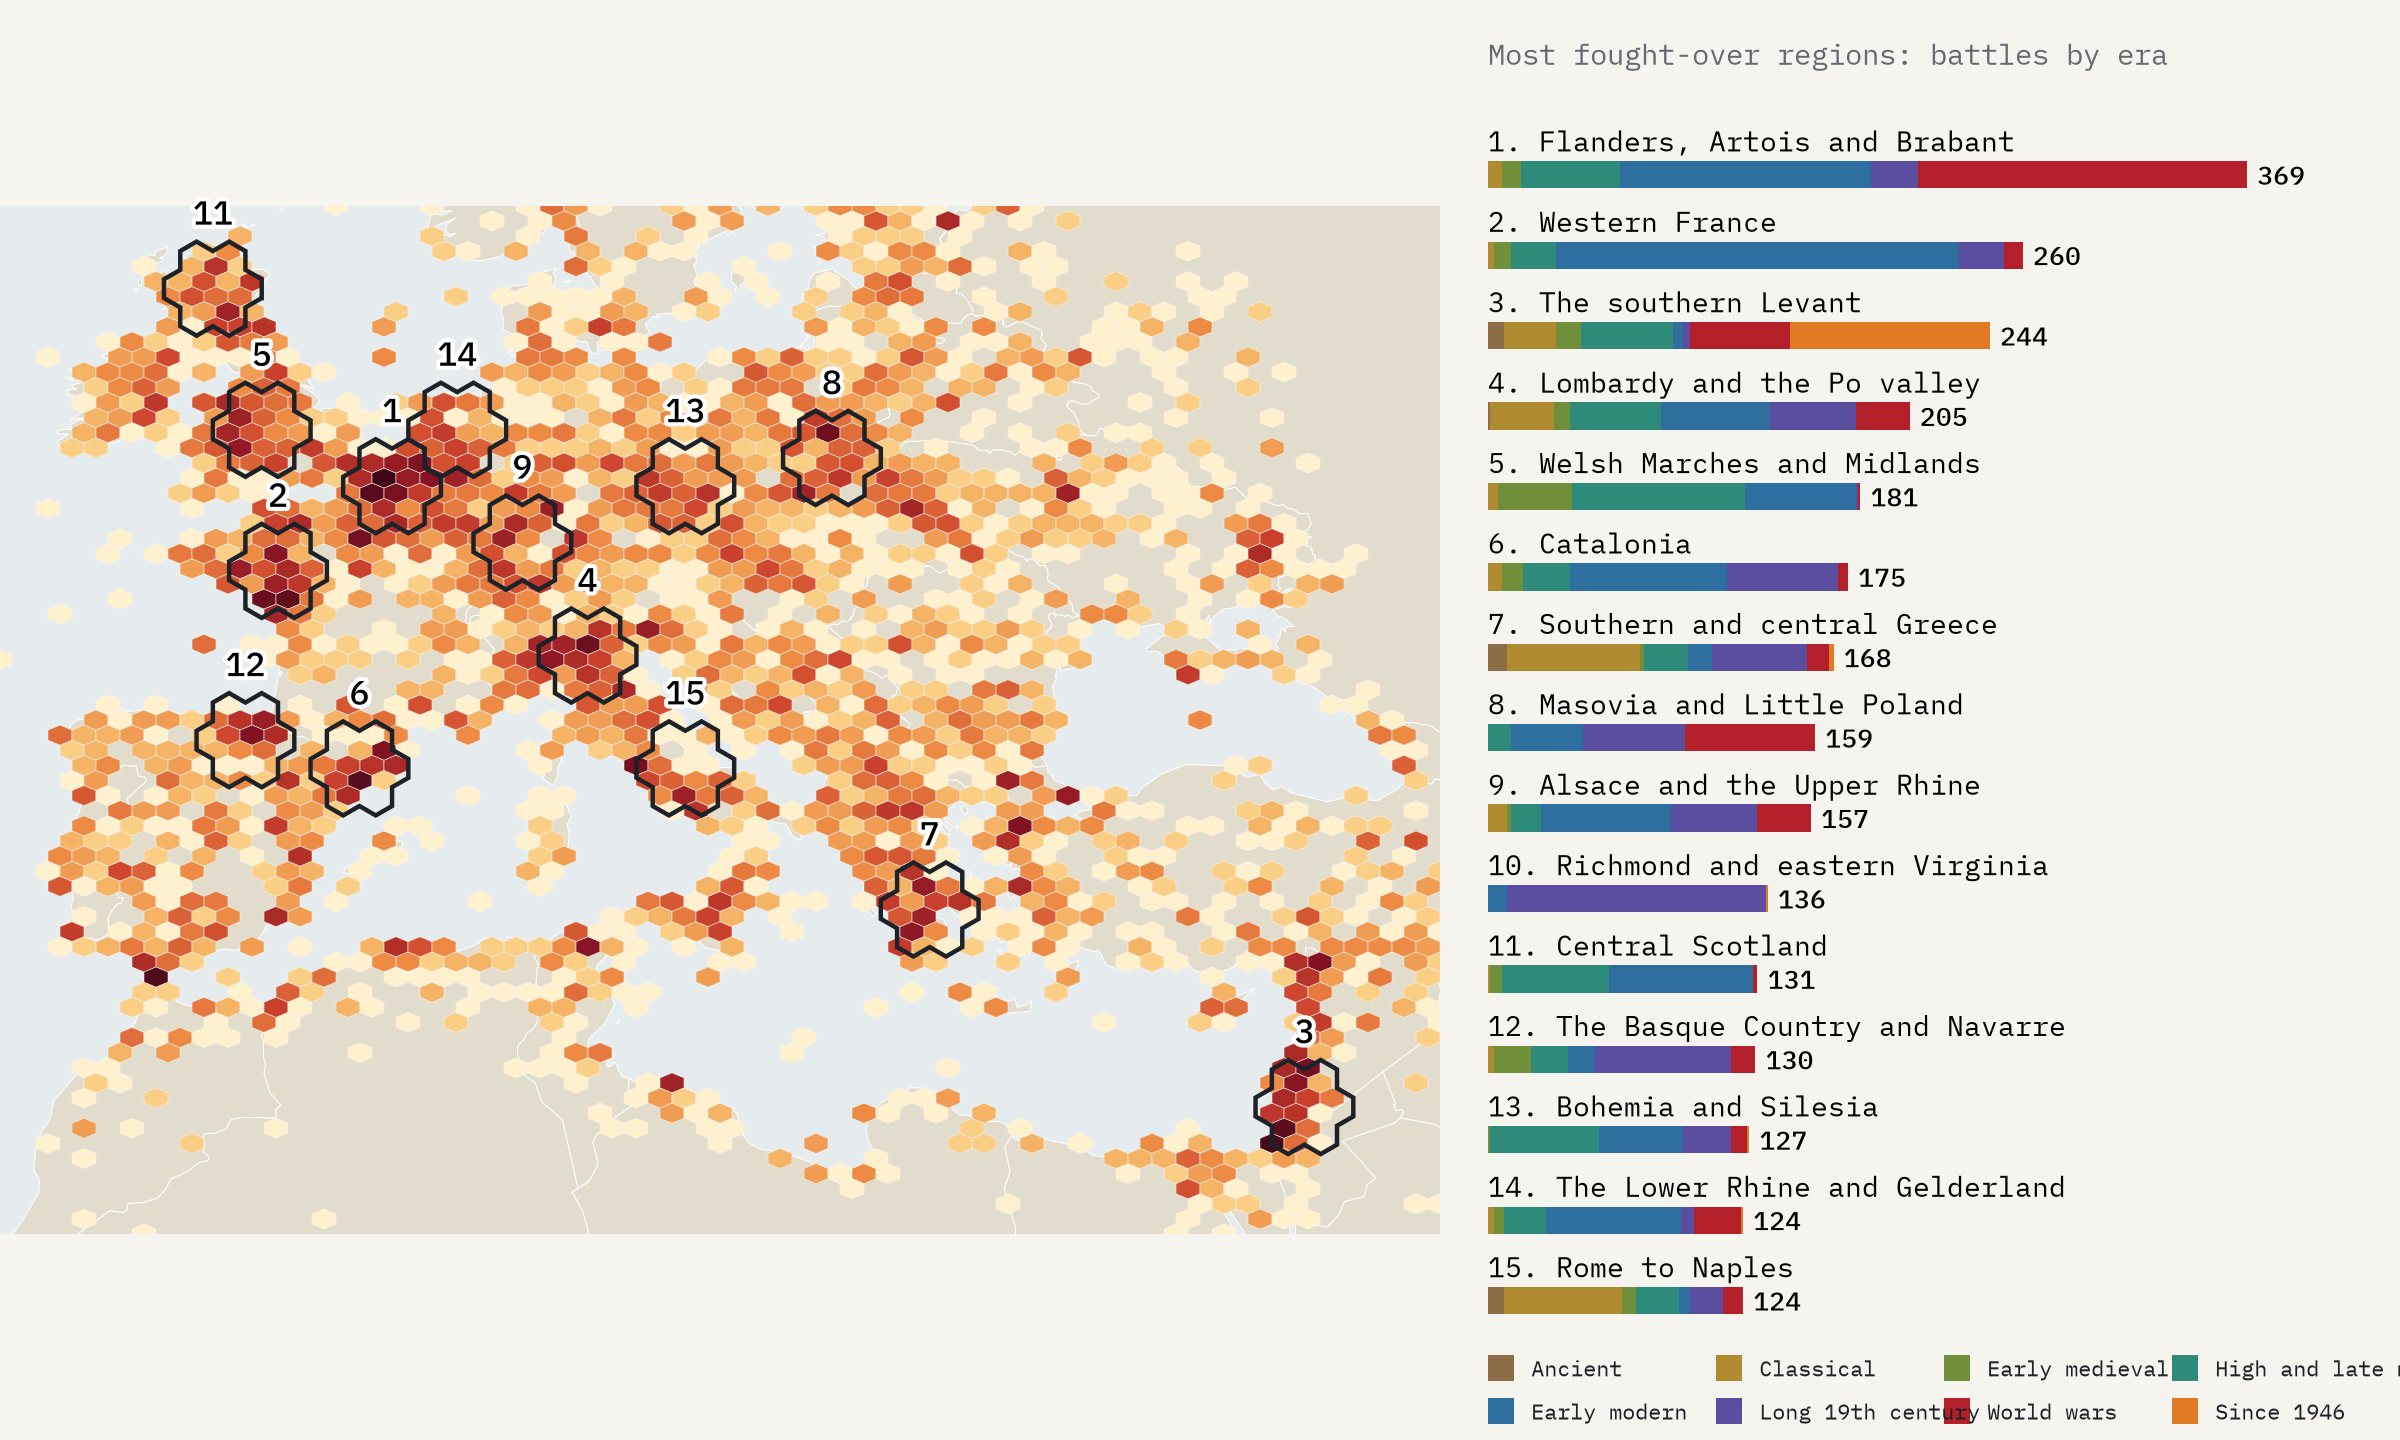
\includegraphics[width=\textwidth]{f_places.png}
\caption{Battles in Europe and the Mediterranean in equal-area hexagons, with the fifteen most fought-over regions of seven hexagons (outlined and numbered; Richmond and eastern Virginia, number 10, is outside the map), and their battles by era.}\label{fig:places}\end{figure}

\begin{table}[tbp]\centering\small\caption{The fifteen most fought-over regions (seven equal-area hexagons, 65,472 km\textsuperscript{2}): battles, centuries with a battle, and the most widely covered battles.}\label{tab:regions}\begin{tabular}{p{4.6cm}rrp{6.4cm}}\toprule Region & Battles & Centuries & Best-known battles\\\midrule
Flanders, Artois and Brabant & 369 & 17 & Battle of Waterloo; Battle of France\\
Western France, from the Vendée to Normandy & 260 & 14 & Falaise Pocket; Battle of Villers-Bocage\\
The southern Levant: Galilee, Jerusalem, Gaza and Damascus & 244 & 21 & Battle of Hattin; Battle of Yarmouk\\
Lombardy and the Po valley & 205 & 22 & Battle of Solferino; Battle of the Trebia\\
The Welsh Marches and the English Midlands & 181 & 16 & Battle of Bosworth Field; Battle of Tewkesbury\\
Catalonia & 175 & 16 & Barcelona May Days; Catalonia Offensive\\
Southern and central Greece & 168 & 21 & Battle of Thermopylae; Battle of Marathon\\
Masovia and Little Poland & 159 & 10 & Battle of Warsaw; Siege of Warsaw\\
Alsace and the Upper Rhine & 157 & 15 & Battle of Ulm; Operation Nordwind\\
Richmond and eastern Virginia & 136 & 4 & Siege of Yorktown; Battle of Chancellorsville\\
Central Scotland and the Highlands & 131 & 14 & Battle of Bannockburn; Battle of Stirling Bridge\\
The Basque Country and Navarre & 130 & 13 & Battle of Roncevaux Pass; Battle of Vitoria\\
Bohemia and Silesia & 127 & 10 & Battle of White Mountain; Battle of Legnica\\
The Lower Rhine and Gelderland & 124 & 14 & German invasion of the Netherlands; Battle of Arnhem\\
Rome to Naples & 124 & 22 & Battle of Monte Cassino; Battle of the Milvian Bridge\\
\bottomrule\end{tabular}\end{table}

\subsection{The best-recorded wars}
66\% of battle items name a war, among 2,166 distinct wars and campaigns (after grouping). The Second World War has 864 battle items, recorded under 60 different ``part of'' values; the First World War has 532 and the American Civil War 524 (Figure~\ref{fig:wars}). The ten best-recorded wars hold 22\% of the battles that name a war. Apart from the Korean, Vietnam, Syrian and Afghan wars, every one of the top 25 was fought mainly in Europe or North America.

\begin{figure}[tbp]\centering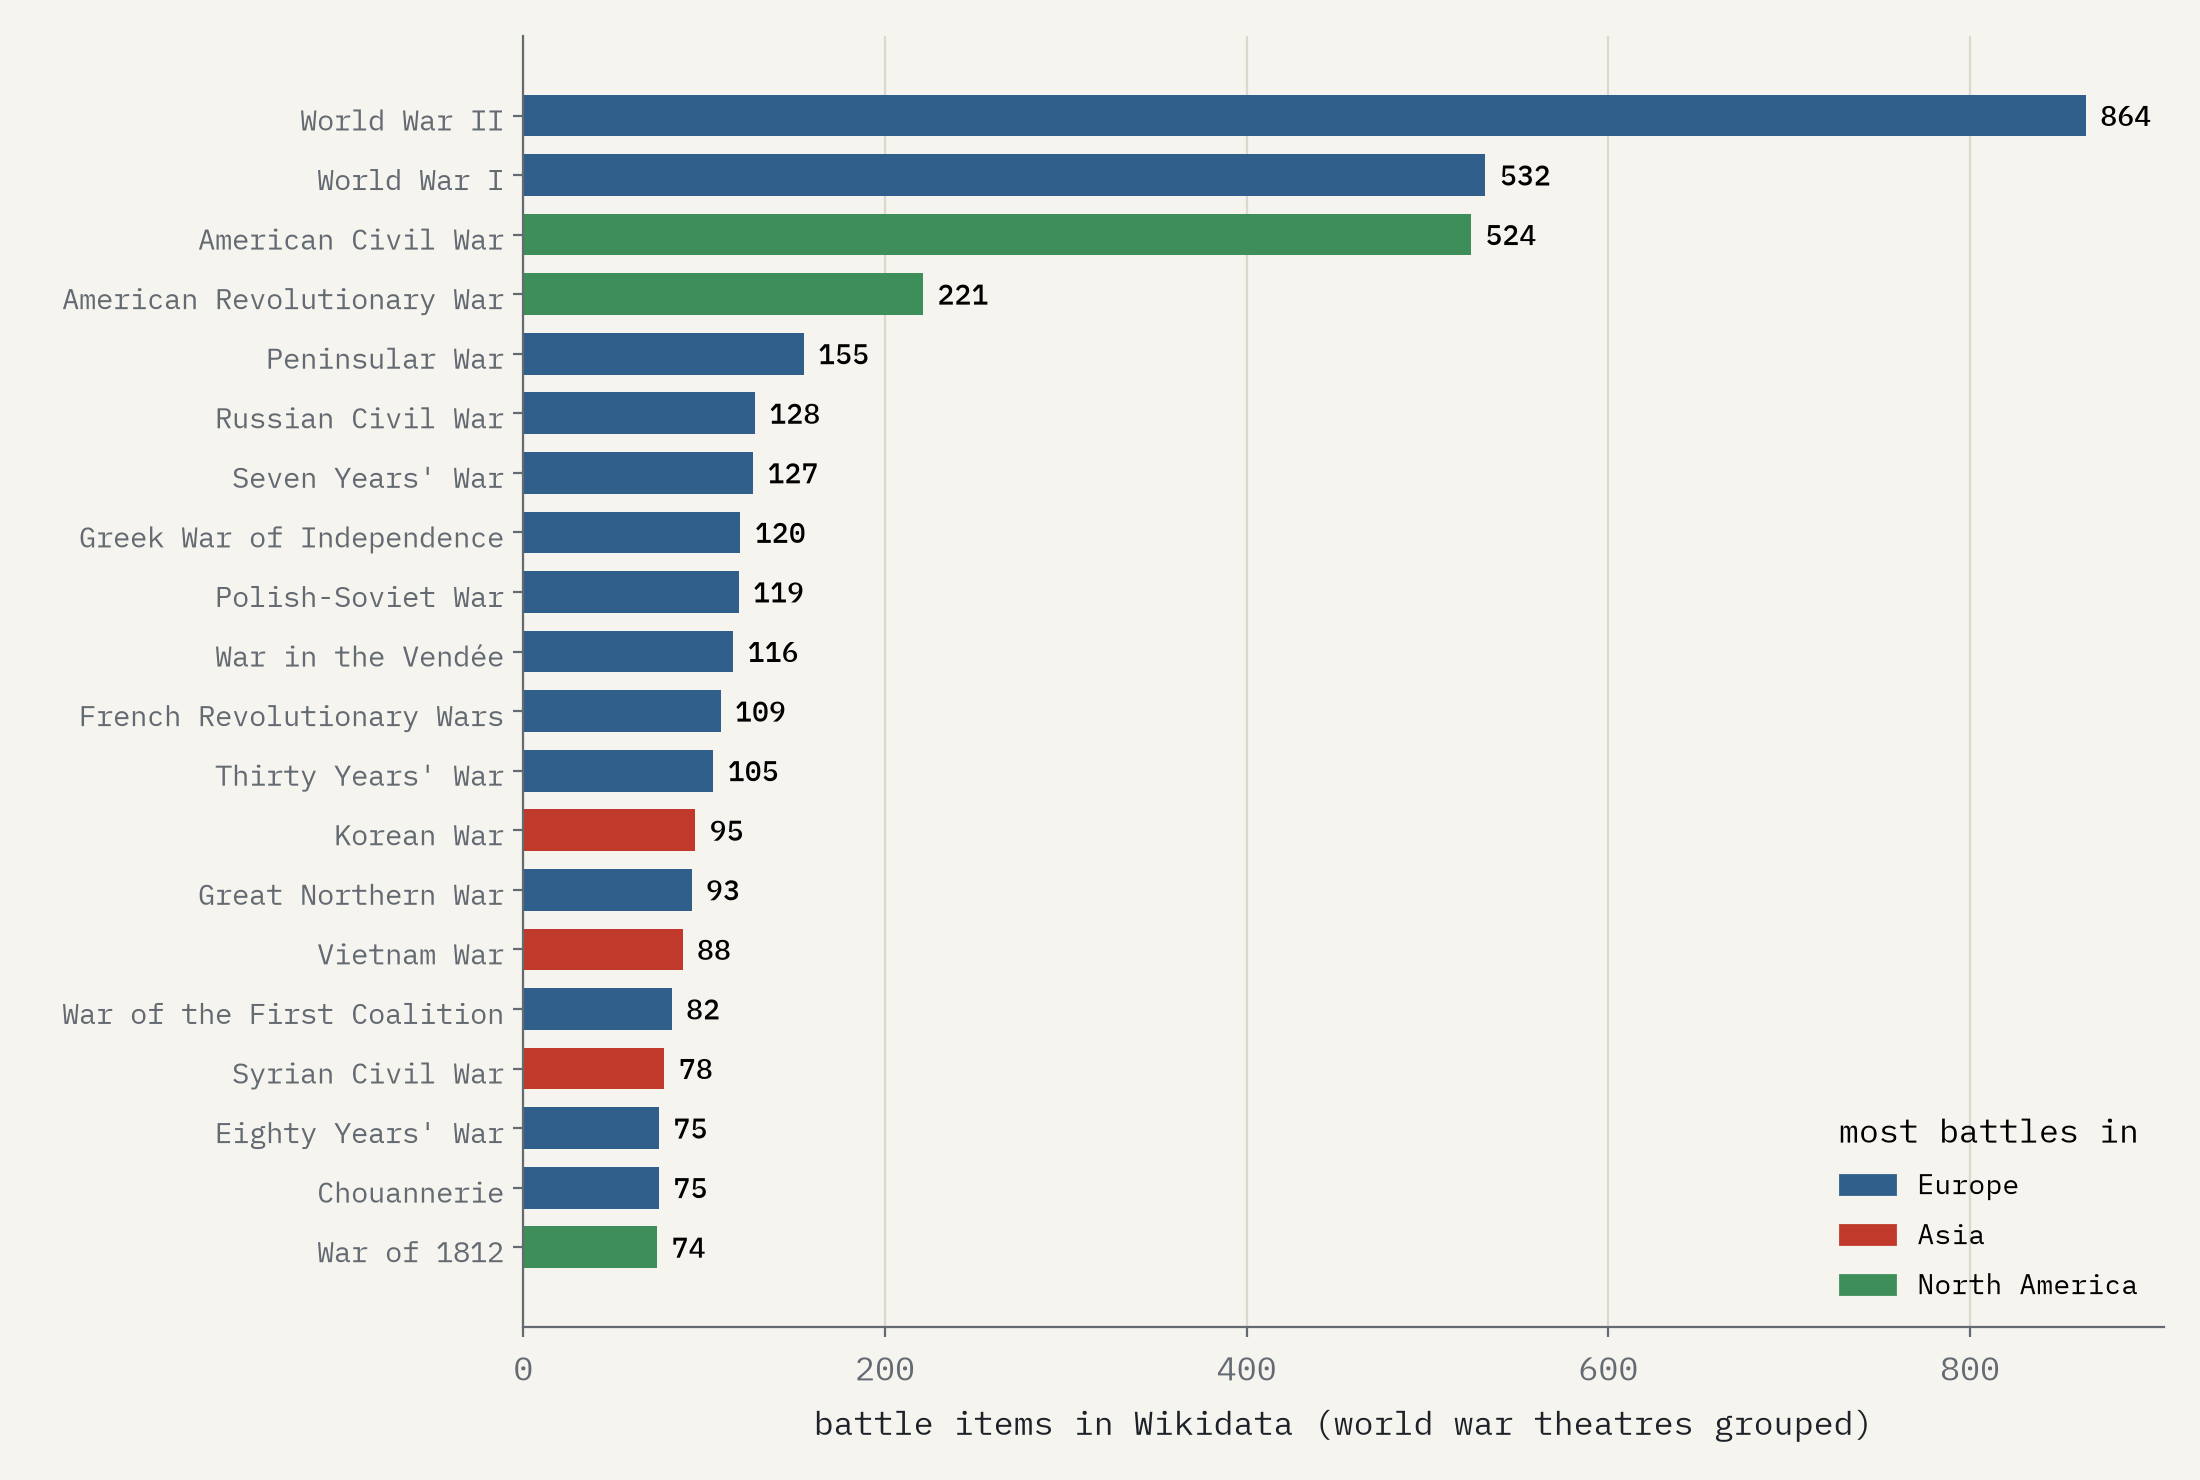
\includegraphics[width=.92\textwidth]{f_wars.png}
\caption{The twenty wars with the most battle items (world war theatres grouped), coloured by the continent with most of their mapped battles.}\label{fig:wars}\end{figure}

\subsection{How skewed is the record?}
Europe has 51\% of mapped battles and 7.4\% of the land outside Antarctica, 6.9 times its share; Asia has 24\% and Africa 9\% (Figure~\ref{fig:bias}). Part of this is real, but a large part reflects how Wikipedia and Wikidata are written. The median battle has 3 sitelinks and 32\% have one or none. Ancient battles in the record are better known than modern ones (median 6 sitelinks before 500 CE against 3 after 1800), a survivorship effect: only famous ancient battles were written about. The most linked are Battle of Stalingrad (108), Battle of Waterloo (95) and Attack on Pearl Harbor (88).

The class itself is inconsistent. Only 79\% of items are labelled as battles in English (Table~\ref{tab:kinds}), and 1,431 (7.1\%) have no English label. Conversely, many major engagements are not typed as battles: only 551 of the 709 rows of Wikipedia's list of battles by casualties (78\%) match a Wikidata battle item, and unmatched rows include Operation Barbarossa, the Siege of Leningrad and the Battle of the Bulge. Among the 540 rows I could map, 63\% are in Europe and 26\% in Asia.

\begin{figure}[tbp]\centering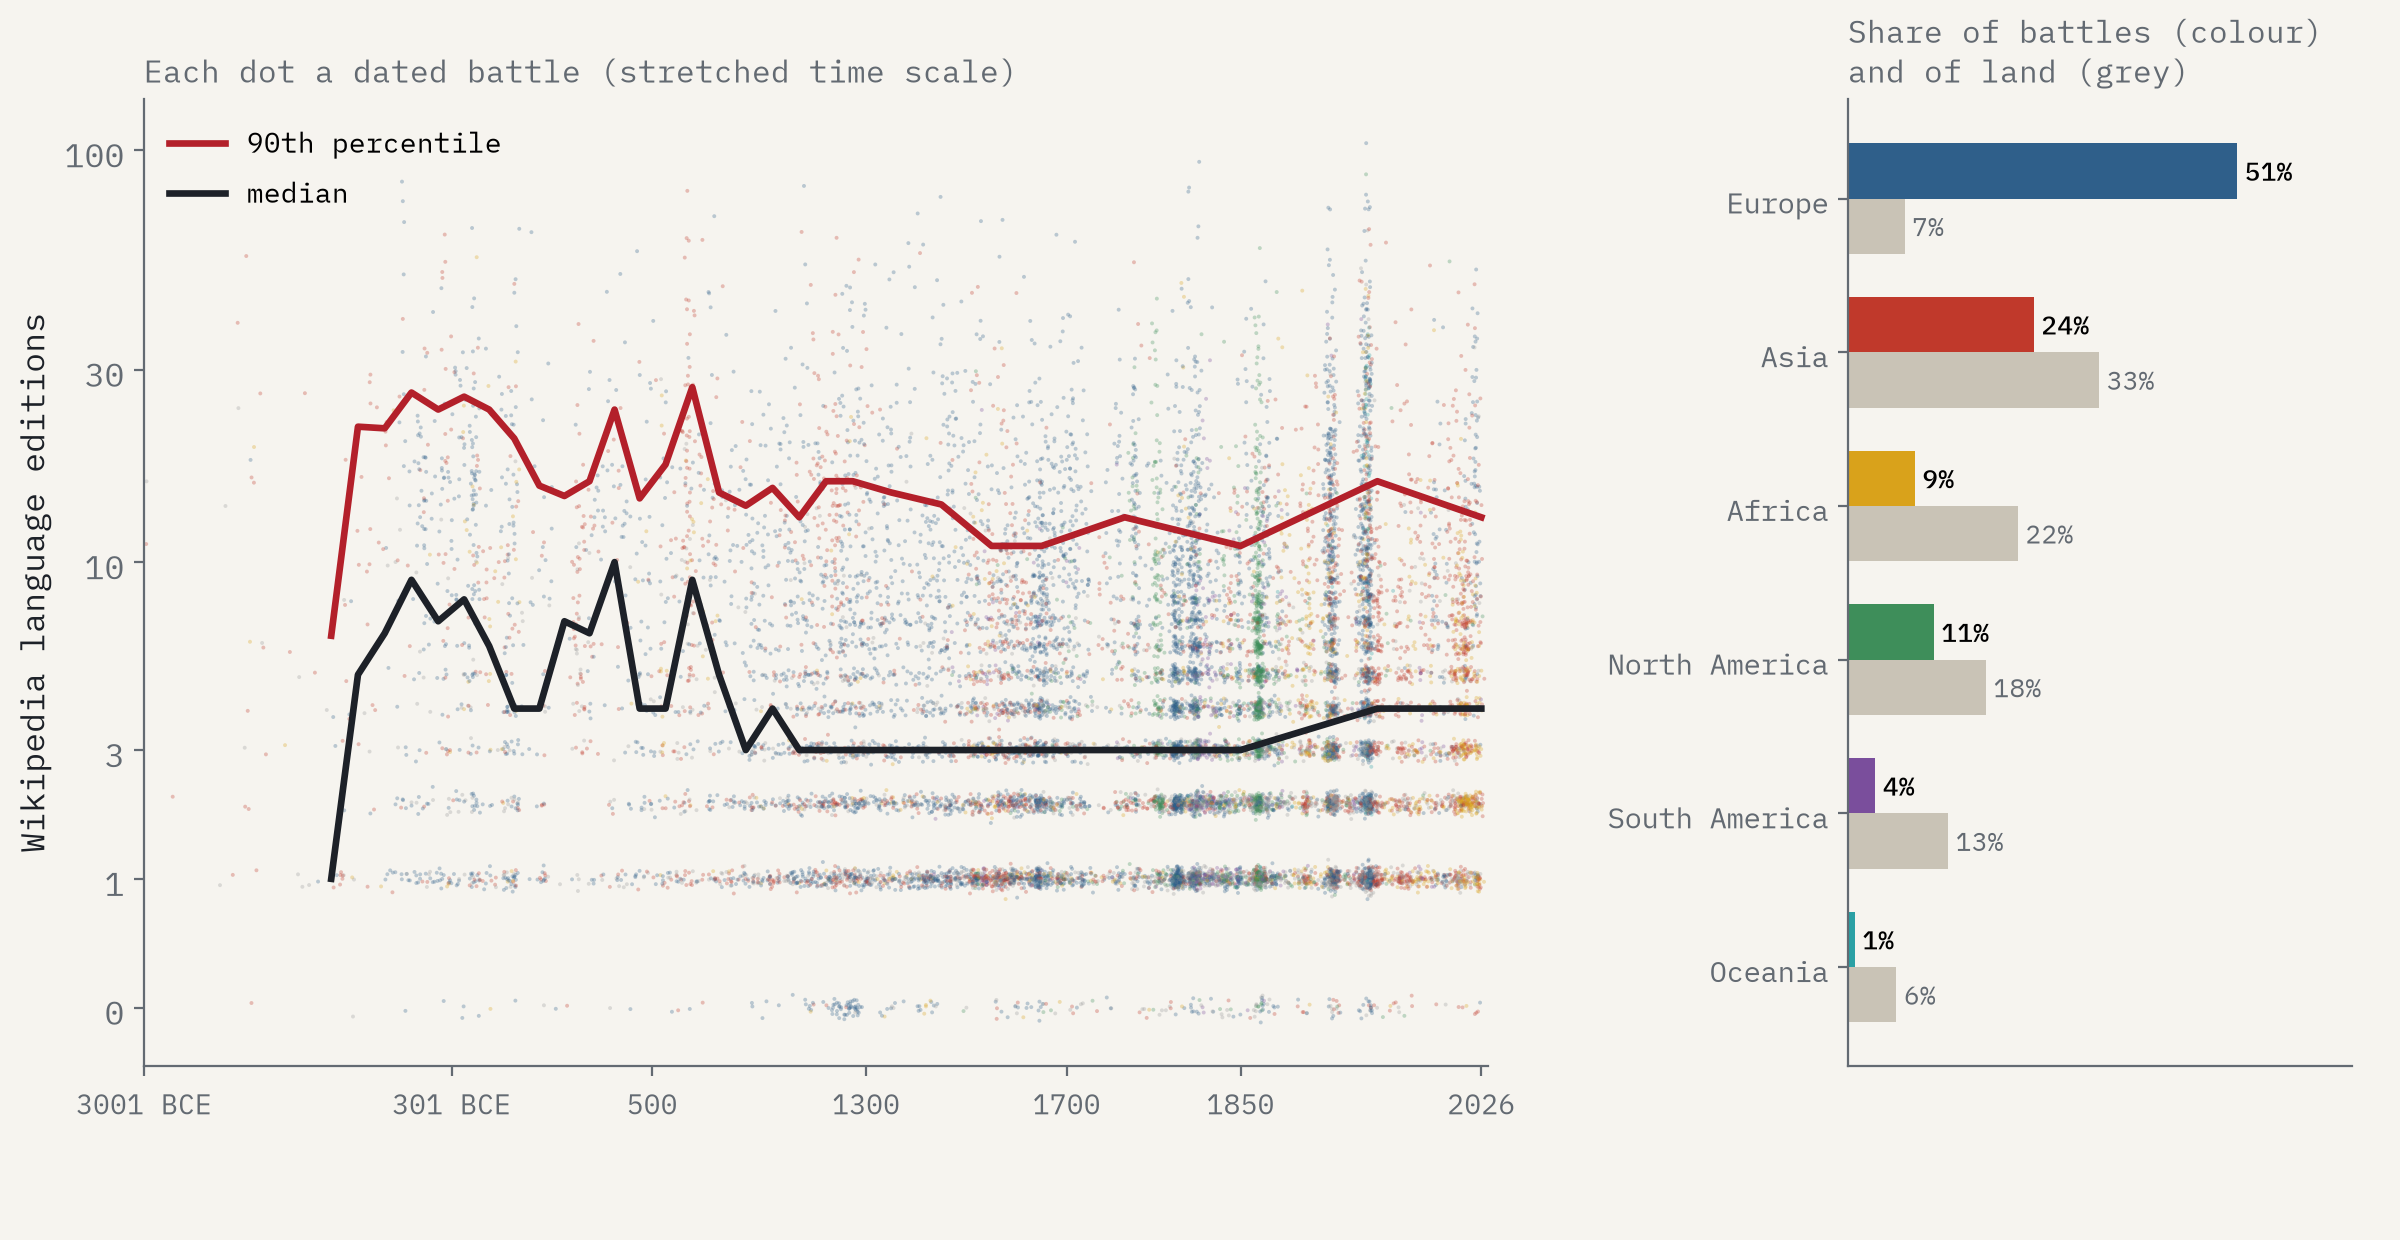
\includegraphics[width=\textwidth]{f_bias.png}
\caption{Left: sitelinks (Wikipedia language editions) of every dated battle against its year on a stretched time scale, with medians and 90th percentiles by century. Right: continents' shares of mapped battles and of land.}\label{fig:bias}\end{figure}

\begin{table}[tbp]\centering\small\caption{Battle items by the first matching word in their English label.}\label{tab:kinds}\begin{tabular}{lrr}\toprule Kind & Items & Share\\\midrule
Battle & 15,910 & 78.8\%\\
Siege & 453 & 2.2\%\\
Skirmish or action & 569 & 2.8\%\\
Raid, attack or capture & 866 & 4.3\%\\
Bombing or bombardment & 18 & 0.1\%\\
Massacre & 32 & 0.2\%\\
Operation or offensive & 510 & 2.5\%\\
Other or no English label & 1,844 & 9.1\%\\
\bottomrule\end{tabular}\end{table}

\section{Discussion}
Read naively, the map says that war has been above all a European affair, that the Vendée was more fought over than China, and that the world became dramatically more violent after 1500. None of these readings is safe. The number of battles recorded for a place and period depends on surviving sources, on the attention of modern historians, and on the work of Wikipedia editors in particular languages. Europe's dominance in the record is partly real, since the continent was densely settled, politically fragmented and very often at war, but it is also the dominance of European historiography and of European-language Wikipedias. The very dense coverage of the American Civil War, the Vendée and the Polish-Soviet War reflects dedicated editing communities.

Some patterns are robust to these caveats. The persistence of the Levant, the Po valley, southern Greece and the land between Rome and Naples as battlefields over two and a half thousand years reflects geography: these are corridors between powers, and places worth holding. Flanders' ranking reflects its position between France, the Low Countries and Germany and its role in the wars of the 17th to 20th centuries. And the movement of the centre of recorded war to the Middle East in the 21st century matches the wars in Syria, Iraq, Yemen and the Sahel, though it also reflects the real-time writing up of recent wars.

\section{Limitations}
First, these are Wikidata items, not battles: there is no complete list of battles against which to measure coverage. Second, the battle class is inconsistent, including sieges, raids and massacres while excluding many offensives and operations, and my classification by label words is rough. Third, coordinates taken from locations can be imprecise, and some ancient battles are legendary or placed by tradition. Fourth, date precision was not available, so ancient years can be approximate; centuries are ordinal. Fifth, the war of a battle depends on how ``part of'' was used, and my grouping covers only the world wars. Sixth, the hexagon and region rankings depend on the grid; the regions reduce but do not remove this. Seventh, casualty figures are Wikipedia's high estimates, frequently disputed, and only matched rows could be mapped. Finally, all counts are for one retrieval in 2026, and Wikidata changes daily.

\section{Conclusion}
A careful map of every battle in Wikidata shows a record that is deep in time but strongly concentrated in Europe and in the last five centuries, a centre of recorded war that stayed near the Alps for two thousand years and has now moved to the Middle East, and a handful of places, Flanders, the Po valley and the southern Levant above all, fought over again and again. It also shows how far such maps describe the historical record rather than war. The interactive version lets readers explore both.

\section*{Data and code availability}
The interactive map is at \url{https://maps.tristanhotham.com/every-battle/}. Data and code are at \url{https://github.com/Tristan-Hotham/every-battle} and archived with this paper at https://doi.org/10.5281/zenodo.23857870. Derived data are released under CC BY 4.0, except the casualty table derived from Wikipedia (CC BY-SA 4.0); code under the MIT licence.

\section*{AI statement}
I wrote the text, with drafting and editing assistance from Claude (Anthropic), which also helped prepare the analysis code. I reviewed and checked all text and results.

\begin{thebibliography}{9}
\bibitem[Bast and Buchhold(2017)]{qlever} Bast, H. and Buchhold, B. (2017) QLever: a query engine for efficient SPARQL+text search. \emph{Proceedings of the 2017 ACM Conference on Information and Knowledge Management}, 647 to 656. \url{https://qlever.cs.uni-freiburg.de/}
\bibitem[Graham et al.(2014)]{graham} Graham, M., Hogan, B., Straumann, R. K. and Medhat, A. (2014) Uneven geographies of user-generated information: patterns of increasing informational poverty. \emph{Annals of the Association of American Geographers}, 104(4), 746 to 764.
\bibitem[Natural Earth(2026)]{naturalearth} Natural Earth (2026) Admin 0 countries (1:50m) and populated places (1:10m). Public domain. \url{https://www.naturalearthdata.com/}
\bibitem[Redi et al.(2020)]{redi} Redi, M., Gerlach, M., Johnson, I., Morgan, J. and Zia, L. (2020) A taxonomy of knowledge gaps for Wikimedia projects. arXiv:2008.12314.
\bibitem[Šavrič et al.(2019)]{equalearth} Šavrič, B., Patterson, T. and Jenny, B. (2019) The Equal Earth map projection. \emph{International Journal of Geographical Information Science}, 33(3), 454 to 465.
\bibitem[Vrandečić and Krötzsch(2014)]{wikidata} Vrandečić, D. and Krötzsch, M. (2014) Wikidata: a free collaborative knowledgebase. \emph{Communications of the ACM}, 57(10), 78 to 85.
\bibitem[Wikipedia(2026)]{wp_cas} Wikipedia contributors (2026) List of battles by casualties. English Wikipedia, revision 1382711824, CC BY-SA 4.0. \url{https://en.wikipedia.org/wiki/List_of_battles_by_casualties}
\end{thebibliography}
\end{document}
